\section{Umsetzung}
\label{sec:Umsetzung}
Nachdem wir in Kapitel \ref{sec:Grundlagen} die theoretischen Grundlagen für unser Vorhaben erläutert haben, wollen wir in diesem Kapitel beschreiben, wie die Grundlagen umgesetzt wurden.

\subsection{Grundlagen zum Elastic Stack}
\label{sub:Grundlagen zum Elastic Stack}
Um die Fragen aus der Problemstellung zu beantworten, wurde der Elastic Stack (ELK) benutzt. Der ELK besteht aus den Software Produkten Elasticsearch, Logstash und Kibana der Firma Elastic N.V. Zusätzlich wurde noch Filebeat von der gleichen Firma benutzt. Die Funktionen der einzelnen Produkte werden in den nachfolgenden Unterkapiteln weiter erläutert. Die folgende Abbildung stellt den Workflow des Systems dar:

\begin{figure}[htb]
\begin{center}
	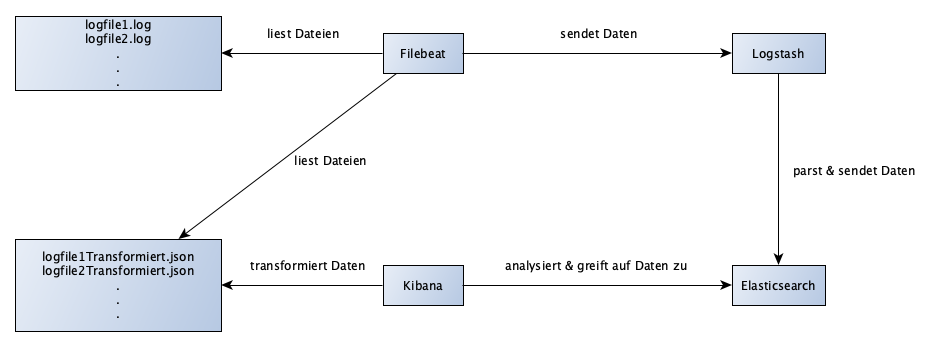
\includegraphics[width=440pt]{bilder/workflow.png}
\end{center}
\caption{ELK Workflow}
\label{fig:elk_workflow}
\end{figure}


\subsubsection{Filebeat}
\label{ssub:Filebeat}
Mit Filebeat können Dateien zeilenweise gelesen werden. In der Konfigurationsdatei von Filebeat gibt man an, wo und nach welchen Dateien gesucht werden soll. In unserem Fall waren es .log und .json Dateien. Außerdem kann man ein multiline pattern angeben, falls ein Eintrag mehrzeilig sein sollte. Die eingelesenen Dateien sendet Filebeat an Logstash weiter. Dabei merkt sich Filebeat, welche Dateien schon gelesen wurden und welche Zeilen in diesen Dateien gelesen wurden. Das bedeutet ebenfalls, wenn eine komplett neue Datei oder eine neue Zeile in einer alten Datei auftaucht, merkt Filebeat das, liest es und sendet die Daten wieder an Logstash. Damit ist die Echtzeitanalyse der Daten gewährleistet. 

\subsubsection{Logstash}
\label{sub:Logstash}
Die Aufgabe von Logstash ist Daten von Filebeat zu empfangen und zu verarbeiten. Die empfangenen Daten befinden sich in einem rohen Zustand und werden mithilfe von mehreren Filter-Plugins verarbeitet.\citep{LoFi20} Nachdem die Daten verarbeitet wurden, sendet Logstash sie weiter an Elasticsearch.

\subsubsubsection{Grok Filter Plugin}\\
Für die Logdateien wurde das Grok Filter-Plugin verwendet. In dem Grok-Filter gibt man einen regulären Ausdruck an, mit dem ein Eintrag in den Logfile gematcht werden soll. Dabei kann man auch direkt festlegen, wie die Daten gespeichert werden sollen, falls gematcht wurde. Allgemein ist die Syntax dabei \%\{REGEXP:Feld\}. Neben einigen regulären Ausdrücken, die im Grok-Filter bereits implementiert sind (wie z.B. \textit{LOGLEVEL, TIMESTAMP\_ISO8601, SPACE, URIPATH}, uvm.), kann man auch eigene reguläre Ausdrücke definieren.
Wie schon in Kapitel \ref{ssub:Segmentierung} beschrieben, sollen die Daten segmentiert werden, was mit dem Grok-Filter realisiert werden kann. So kann man z.B. duch richtiges Platzieren von \textit{Incoming Request} in dem regulären Ausdruck erreichen, dass \textit{Outgoing Responses} nicht gematched und dadurch auch nicht weiter beachtet werden. Außerdem ist es möglich Daten matchen, aber keinem Feld zuweisen, wodurch sie auch nicht gespeichert werden.\\
Weiterhin hat man die Möglichkeit, die Felder, die durch das Matching mit dem regulären Ausdruck mit Daten gefüllt werden, weiter zu bearbeiten. Dafür können wiederum verschiedene Filter benutzt werden. So hat man die Möglichkeit Felder, die Logstash automatisch anlegt, zu bearbeiten. Ein praktisches Beispiel hierfür ist der \textit{date}-Filter: Logstash legt automatisch ein Feld für einen Zeitstempel an, der auf den Moment eingestellt ist, an dem Logstash den eingehenden Eintrag verarbeitet. Mit dem date-Filter hat man die Möglichkeit dieses Datum zu manipulieren. In unserem Fall wurde nicht der aktuelle Zeitstempel benutzt, die Einträge zu speichern, sondern der Zeitstempel aus dem Logeintrag. Das hat den Vorteil, dass man nicht zwei verschiedene Zeitstempel speichern muss.

\subsubsubsection{Ruby Filter Plugin}\\
%\\
Das Ruby Filter Plugin wird benutzt, um transformierte Daten in Elasticsearch zu speichern. An dieser Stelle sei angemerkt, dass Elasticsearch zwar eine experimentelle \textit{transform} Funktion besitzt, diese aber für unseren Anwendungsfall (noch) nicht passend implementiert ist \citep{ElTr20}. Deshalb wurde ein Ruby Skript entwickelt, das diese Funktion ergänzt.\\
Das entwickete Skript liest aus JSON Dateien die Session Entities ein, die in Kapitel \ref{ssub:Feature_extraction} vorgestellt wurden. Wie genau diese Daten aussehen bzw. wie sie zustande kommen, wird in Kapitel \ref{ssub:Kibana} genauer erläutert. Zum besseren Verständnis, wie das Ruby Skript arbeitet, wird an dieser Stelle daher die Datenstruktur abstrakt beschrieben.
Im Prinzip sind die Daten in drei Ebenen aufgeteilt:\\
\begin{enumerate}
	\item UserIDs
	\item SessionIDs
	\item Widgets
\end{enumerate}
Dabei kann man jeweils eine Ebene als ein Array betrachten. So besteht die oberste Ebene aus einem Array, das mit UserIDs gefüllt ist. Zu der UserID wird zusätzlich ein Array gespeichert, das aus SessionIDs besteht, die zu der UserID gehören. Zu diesen SessionIDs wird schließlich ebenfalls ein Array verknüpft, in dem festgehalten wird, welche Widgets in der Session genutzt wurden und wie oft. Nun durchläuft das Skript also die beschriebenen Array Ebenen und speichert die gegebenen Daten in passende Felder. Die Daten werden schließlich an Elasticsearch gesendet und dort in einem passenden Index gespeichert.\\
Erwähnenswert ist noch, dass wir die transformierten Daten allerdings auf zwei Arten verarbeitet werden mussten. Die Gründe dafür werden in Kapitel \ref{ssub:Kibana} genauer erläutert.

\subsubsection{Elasticsearch}
\label{ssub:Elasticsearch}
Nachdem die von Filebeat gelesenen Daten von Logstash geparst wurden, werden die Daten in Elasticsearch gespeichert. Dabei werden die Logeinträge und die transformierten Daten separat indiziert. Die Daten, die an Elasticsearch gesendet werden, können automatisch gemapped (also einem Datentyp zugeordnet) werden. Das heißt, Elasticsearch erkennt, ob z.B. ein Datum oder eine Zahl gespeichert wurde. Des Weiteren hat man aber auch die Möglichkeit, ein eigenes Mapping zu definieren. Nachdem aber ein Mapping in dem Index gespeichert wurde, kann es nicht mehr ohne weiteres geändert werden.\\
Für das weitere Verständnis ist es notwendig zu beschreiben, wie unsere Daten in Elasticsearch gespeichert werden. Um aber nicht unnötig ausschweifend zu werden, beschränken wir uns nur auf die Aspekte, die für uns relevant sind.\\
Allgemein werden Daten in Elasticsearch in Indizes gespeichert. Diese Indizes sind eine Sammlung von Dokumenten, in denen die gespeicherten Daten stehen. Die Daten sind als Key-Value-Paare gespeichert. \begin{comment}Trotz das Elasticsearch keine relationale Datenbank ist, werden die vorgestellten Begriffe zu ihren Gegenstücken einer relationalen Datenbank zugeordnet:

\begin{table}[htb]
	\centering
	\begin{tabular}{l|p{3cm}}
		relationale Datenbank & Elasticsearch\\ \hline
		Tabelle & Index\\
		Spalte & Dokument\\
		Zeile & Feld
	\end{tabular}
	\caption{Vergleich relationale Datenbank vs. Elasticsearch}
	\label{tab:rdb_vs_el}
\end{table}
\end{comment}
\subsubsection{Kibana}
\label{ssub:Kibana}
Kibana ist ein Tool, um die Daten, die in Elasticsearch gespeichert sind, zu visualisieren bzw. zu analysieren. So kann man bspw. mit wenigen Einstellungen Visualisierungen der in Elasticsearch gespeicherten Daten erstellen, welche man wiederum zu einem Dashboard zusammen fassen kann. Ferner bietet Kibana die Möglichkeit, die Daten auch manuell zu durchsuchen. Sollte Kibana eine gewünschte Visualisierung oder ein gewünschtes Analysetool nicht nativ enthalten, hat man die Möglichkeit es um die gewünschten Funktionen zu erweitern.\\
Für unsere Anwendung ist eben dieser Fall eingetreten, da man nicht ohne weiteres Assoziationsregeln mit Kibana finden kann.\\
Bevor wir darauf eingehen, wie das Custom Plugin und die Visualisierungen eingesetzt wurden, wollen wir den Hinweis aus Kapitel \ref{sub:Logstash} aufgreifen und erläutern, warum es notwendig war, die transformierten Daten in separaten Indizes zu speichern. Wie schon erwähnt wird zu einer SessionID ein Array gespeichert, das Informationen zu den benutzten Widgets enthält. In Elasticsearch kann man Arrays unter dem Datentyp \glqq nested \grqq{} speichern. Allerdings ist es in den Visualisierungen, die für unsere Zwecke relevant sind, nicht möglich, Daten in einer verschachtelten Datenstruktur zu lesen bzw. zu durchsuchen. Also müssen die Einträge zu den transformierten Daten in einzelnen Dokumenten in Elasticsearch gespeichert werden.\\
Für die Suche nach Assoziationsregeln ist diese Datenstruktur aber nicht geeignet. Möchte man z.B. nach den Sessions suchen, in denen zwei bestimmte Widgets benutzt wurden, schlägt die Suche fehl. Die Begründung dafür ist, dass in den Dokumenten nur ein Widgetname steht, aber Elasticsearch nach zwei suchen würde. Deshalb müssen die Session Entities sowohl in der Array Variante gespeichert werden, als auch als Dokumente, die nur einen Widgetnamen beinhalten.

\subsubsubsection{Custom Plugin}\\
Um einen erleichterten Einstieg in die Entwicklung eines Custom Plugins zu ermöglichen, bietet Kibana die Möglichkeit, das Grundgerüst für ein Custom Plugin generieren zu lassen. Das generierte Plugin liefert direkt die nötige Server-Client-Architektur, um den Elasticsearch-Server anzusprechen. Die grafische Oberfläche, die der Nutzer sieht, ist dabei als Client zu verstehen. Von hier aus werden HTTP Requests an einen Node.js Server gesendet. Dieser kann nun die gesendeten Daten (bspw. eine Suchanfrage) vorbereiten, an den Elasticsearch-Server senden, die Antwort verarbeiten und an den Client weiterleiten. Außerdem ist der Node.js Server auch in der Lage, Python Code ausführen zu lassen. Die folgende Abbildung soll diese Beziehung verdeutlichen. 
\begin{figure}[htb]
\begin{center}
	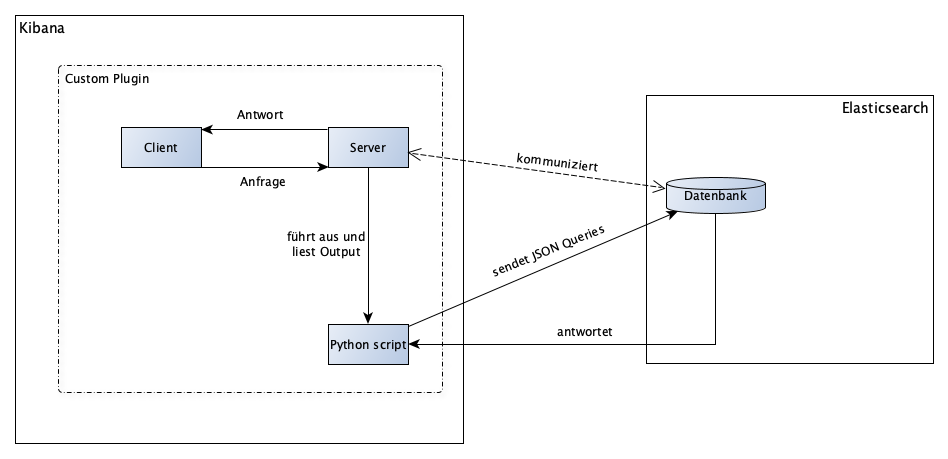
\includegraphics[width=430pt]{bilder/custom_plugin.png}
\end{center}
\caption{Architektur des Custom Plugins}
\label{fig:custom_plugin}
\end{figure}


\subsubsubsection{Visualisierungen}
%\textbf{Visualisierungen}\\
\\
In dieser Arbeit wurden zwei Visualisierungen benutzt, die in Kibana bereits integriert sind: die \textit{Pie} und \textit{Line} Visualisierungen. Erstere wurde benutzt um festzustellen, zu welchen Anteilen die zufälligen Widgeteinträge generiert wurden.\\
Die \textit{Line} Visualisierung wurde benutzt, um die erste Frage aus Kapitel \ref{sub:Problemstellung} zu beantworten. Die Visualisierung zeigt in einem zweidimensionalen Diagramm die Benutzung der Widgets über einen bestimmten Zeitraum, wobei dieser Zeitraum auf der x-Achse abgebildet wird. Die y-Achse gibt die Anzahl an Widget Nutzungen an. Das bedeutet ein Punkt in dem Diagramm zeigt an, wie oft ein Widget an einem bestimmten Tag benutzt wurde. Schließlich verbindet die Visualisierung die Punkte miteinander und so erhält man eine Linie, die der Widgetnutzung in einem bestimmten Zeitraum entspricht. Abbildung \ref{fig:screen_lines} zeigt wie die Visualisierung beispielsweise aussehen könnte.

\begin{figure}[htb]
\begin{center}
	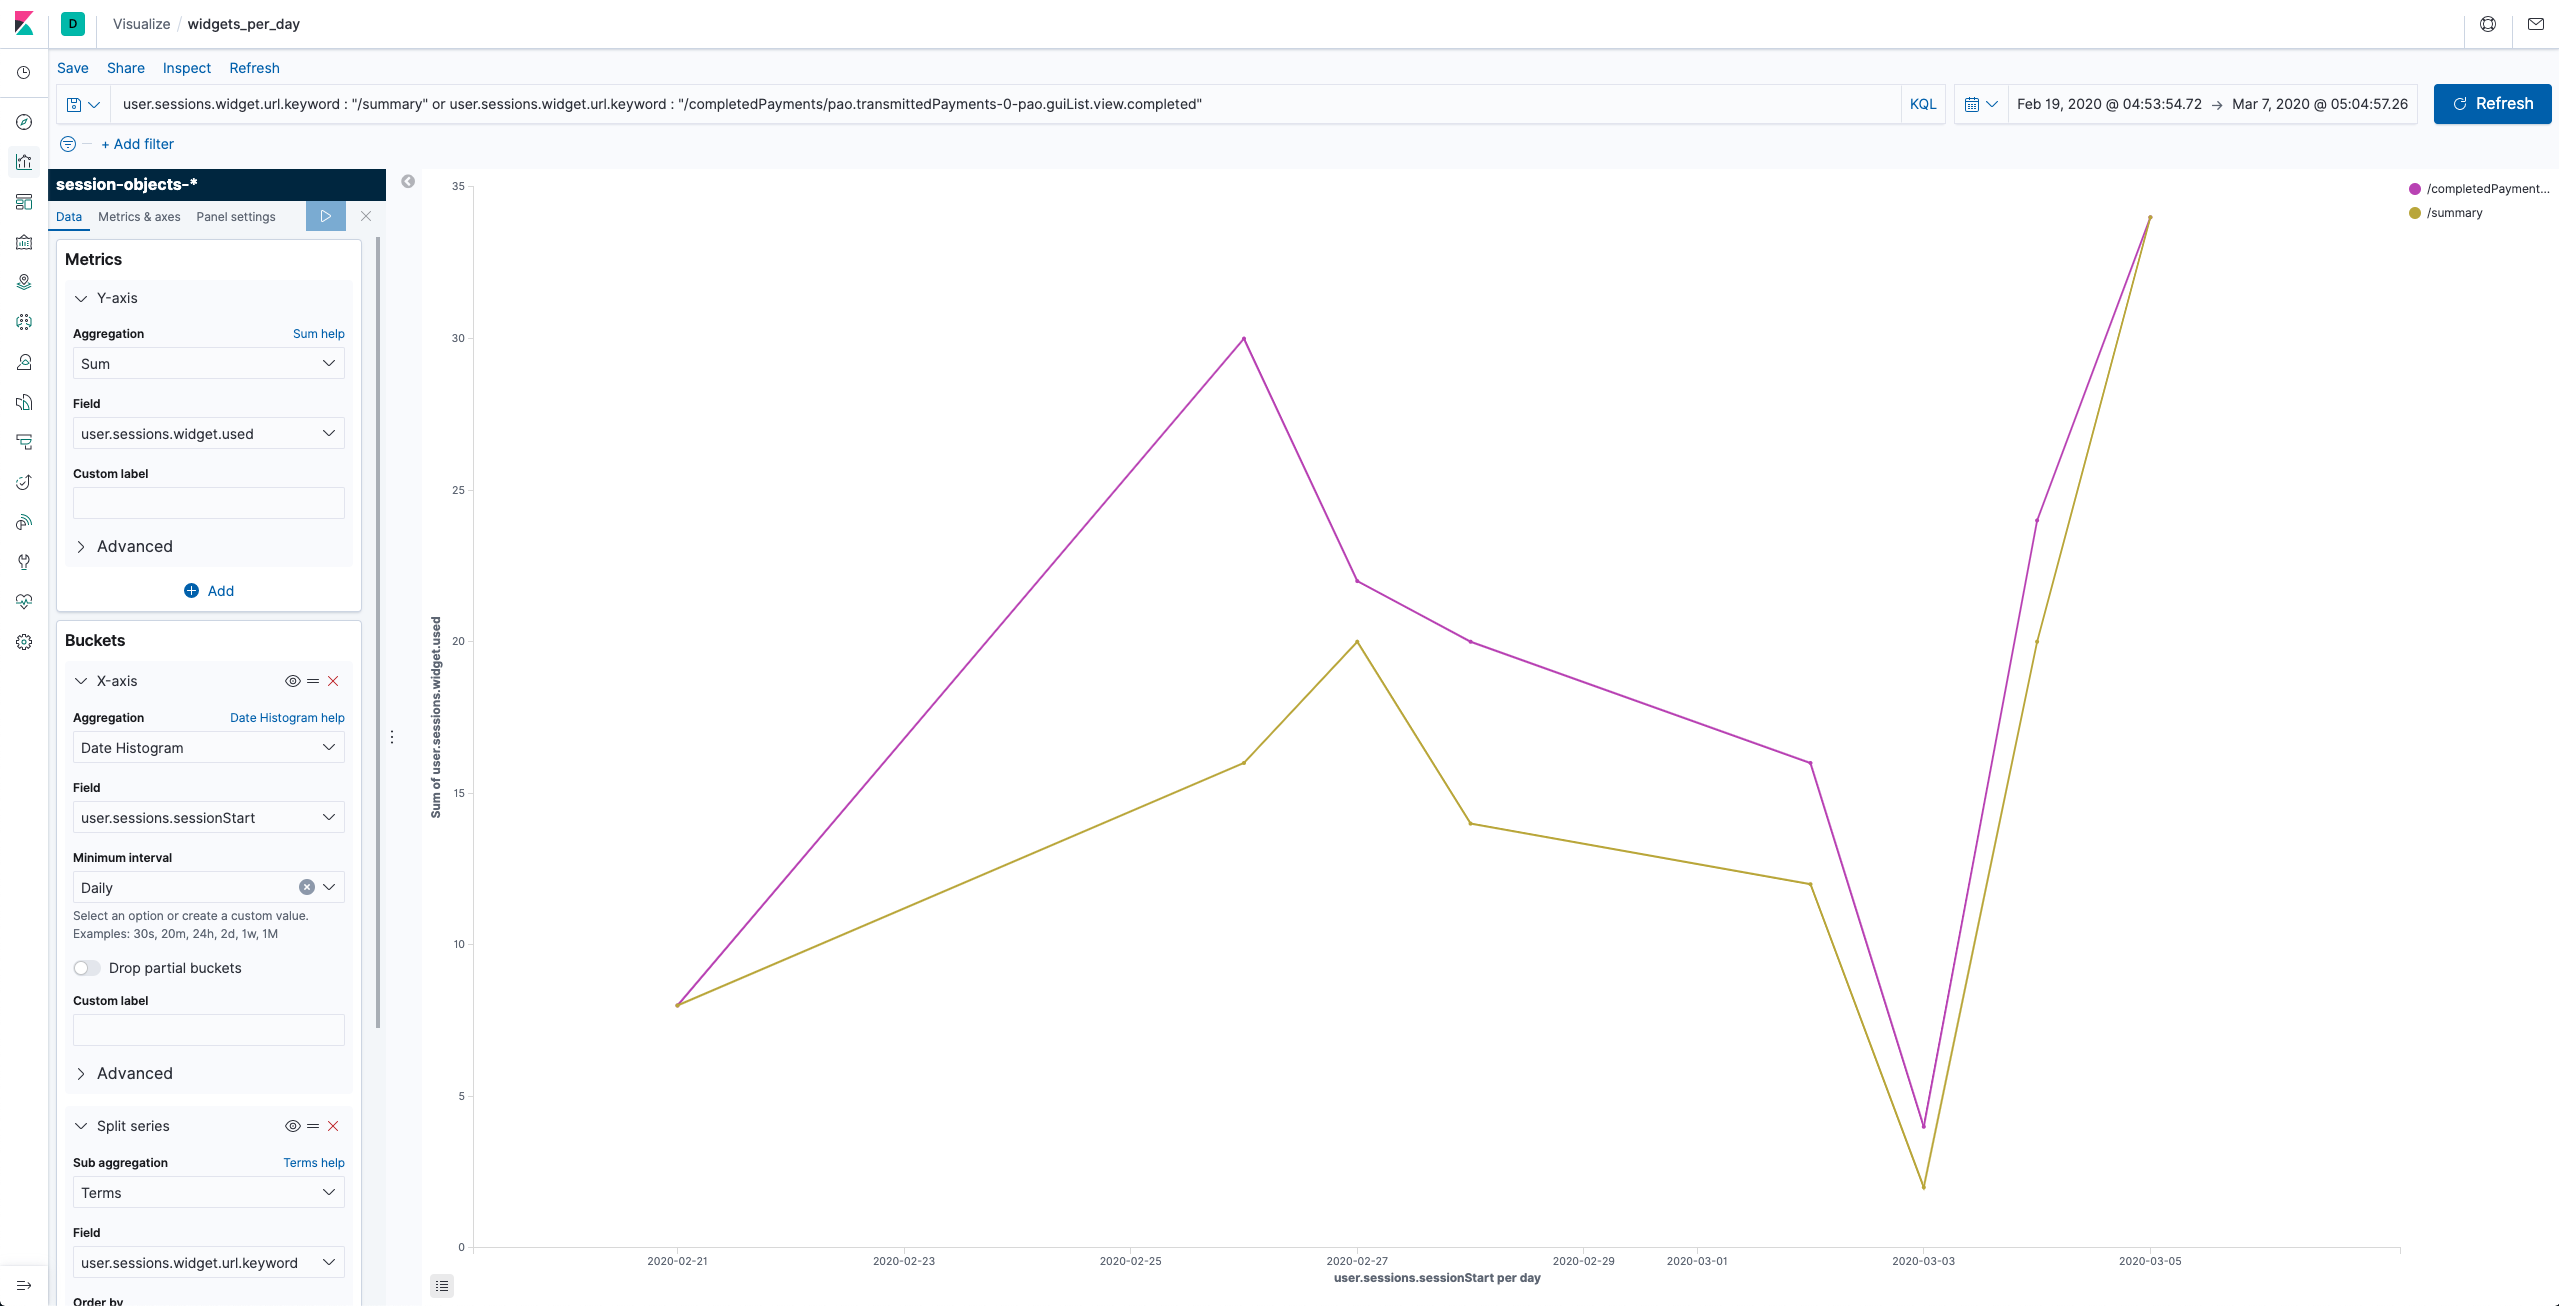
\includegraphics[width=430pt]{bilder/screen_lines.png}
\end{center}
\caption{Lines Visualisation mit zwei Widgets}
\label{fig:screen_lines}
\end{figure}


%\textbf{Custom Plugin}\\\\
%Kibana bietet aber nicht ohne Weiteres die Möglichkeit, einen Workflow zu erkennen, wie es in der zweiten Frage aus Kapitel \ref{sub:Problemstellung} gefordert ist. Deshalb wurde im Zuge der Arbeit ein Custom Plugin für Kibana entworfen.


\clearpage
